
\chapter{Digital Measurement}\label{c:measure}
\section{Telling Tall Tales}
The first thing that comes to mind when we mention measurement is often the lowly ruler.  Because of its familiarity, the ruler is a nice place to start our conversation about the basic characteristics of measurement.

Imagine you have just caught a large fish from your local pond/lake/stream/ocean.  Because you practice catch-and-release (of course) you'll want to measure the length of your catch to avoid an common accusation of telling tall tales.  First you'll need to find an appropriately sized ruler to make the measurement.  The size of the ruler will dictate the \gls{range} of the measurement.  Were you fishing for Brook Trout or a Blue Marlin?  Hopefully you brought along a ruler with a range that exceeds the maximum predicted length of your catch, otherwise you'll have to resort to extrapolation!

Once we lay our ruler alongside our catch we'll need to estimate the actual length based on the graduation marks on the ruler.  The distance between these marks is the \gls{resolution} of our measurement, which is the smallest step size available.  The finest marks on a typical yardstick might be one-half inch, so our resulting measurement would have a resolution of \unit[0.5]{in}.  If we have a large set of calipers, the resolution of our measurement would be more like \unit[0.001]{in}.

Finally, when we are back on land and telling our tale we will inevitably be challenged on the \gls{accuracy} of our measurement which can attempt to quantify using the \gls{error} (E)
\begin{equation}
E = \mathrm{measured value} - \mathrm{true value}.
\end{equation}
This is a difficult calculation to do without knowing the ``true'' length of our fish, but we'll return to that topic later.

\section{Bits and Bytes}
In a moment we'll discuss how we might make this measurement using a digital device, but, as an aside, we'll need to introduce the basics of \gls{binary numbers}.  The base-2, or binary, number system represents numbers using two symbols: 0 and 1.  This number system is the foundation for all digital electronics, including computers.  

One way to describe the binary system is to compare it to the base-10, or decimal, number system that most of us are more familiar with.  Each binary digit is called a \gls{bit} and can be 0 or 1.  If we want to be able to count higher than 1, we need to combine multiple bits to represent an integer.

\begin{table}[bt!] 
\renewcommand{\arraystretch}{1.2}
\caption{Four-bit binary number examples}
\label{t:binary}
\centering
\begin{tabular}{|c|c|c|c||c|}\hline
MSB &\hspace{4ex} & \hspace{4ex}& LSB & Base-10\\ \hline \hline
$2^3$ & $2^2$ & $2^1$ & $2^0$ & \\ \hline \hline
0 & 0 & 0 & 0 & 0 \\ \hline
0 & 0 & 0 & 1 & 1 \\ \hline
0 & 0 & 1 & 0 & 2 \\ \hline
0 & 0 & 1 & 1 & 3 \\ \hline
0 & 1 & 0 & 0 & 4 \\ \hline
0 & 1 & 0 & 1 & 5 \\ \hline
\end{tabular}
\end{table}

Table~\ref{t:binary} illustrates how a 4-bit binary number can be used to represent an integer number.  For this example we have placed the most significant bit (MSB) on the left side and the least significant bit (LSB) on the right so that the number is read similar to how we write decimal numbers (the 10's place goes to the right of the 1's place). To convert from the binary representation (the four columns on the left) to the base-10 represenation we can take each binary digit (bit) and multiply by the second row.  For example, for the sixth row in the Table~\ref{t:binary} we see
\[
0*(2^3)+0*(2^2)+1*(2^1)+1*(2^0) = 2+1 = 3.
\]

\begin{ex}
What is the largest decimal integer (base-10) that can be represented by a 4-bit binary number?  (See Table~\ref{t:binary})  Write the integer in both binary (base-2) and decimal (base-10) forms.
\end{ex}

\ifsolutions

\begin{soln}
See Table~\ref{t:binarys}.  The maximum number we can represent is 15.  The minimum number is 0.
\begin{table*}[bt!] 
\renewcommand{\arraystretch}{1.2}
\caption{Solution}
\label{t:binarys}
\centering
\begin{tabular}{|c|c|c|c||c|}\hline
MSB &\hspace{4ex} & \hspace{4ex}& LSB & Base-10\\ \hline \hline
$2^3$ & $2^2$ & $2^1$ & $2^0$ & \\ \hline \hline
1 & 1 & 1 & 1 & 1 \\ \hline
\end{tabular}
\end{table*}
\[ (1)*2^3+(1)*2^2+(1)*2^1+(1)*2^0 = 15 \]

\end{soln}

\fi


The number of bits determines the number of integers that can be represented.  For a 1-bit number can represent $\{0,1\}$, a 2-bit number can represent $\{0,1,2,3\}$, a 3-bit number can represent $\{0,1,2,3,4,5,6,7\}$, etc.  Finally, an M-bit number can represent $2^M$ in integers.  

\section{The Digital Ruler}
Now we can return to our fishing expedition.  This time, instead of a regular (analog) ruler, we have a digital meter stick.  This magical instrument is one meter long (so the full scale range (FSR) is \unit[1.0]{m}) and it reports the length of the fish as a 3-bit number.  Figure~\ref{f:fish} illustrates our measurement.
\begin{figure}[hbt!]
\centering
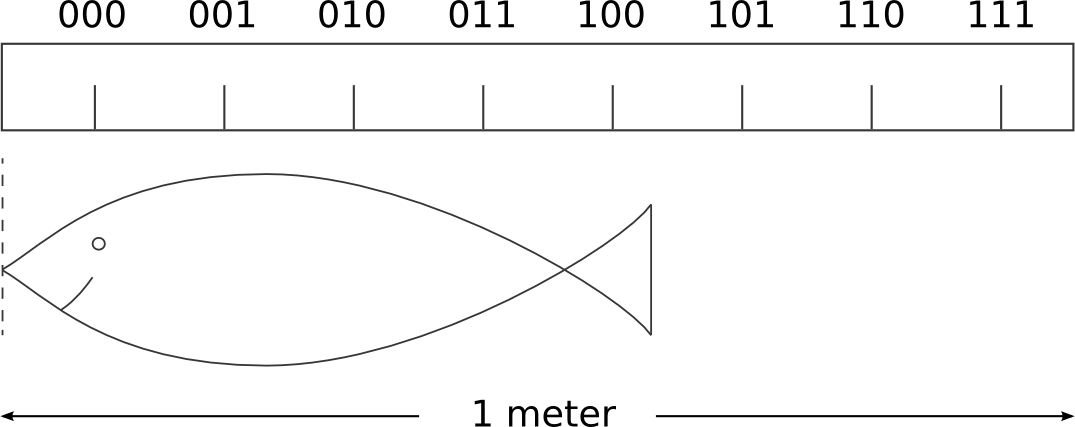
\includegraphics[width=\FigWidth\textwidth]{fish.png}
\caption{Measuring our catch with a digital ruler.}
\label{f:fish}
\end{figure}

Remember, that our digital ruler can only report a 3-bit number.  From the illustration we might anticipate that the ruler would report the binary number $100$ since that is closest to the actual length of our fish.  However, since most of our friends are engineers, they will expect our fishing story to have engineering units.  How do we convert this binary number to an actual length?

Since we know the range of our measurement (\unit[1.0]{m}) and the total number of bits (3) we can convert to a length ($L$) using a ratio
\begin{equation}
L = FSR \left(\frac{X}{2^M - 1}\right
) = (1.0 m)(4/7) = 0.57 m
\end{equation}
where $X$ is the decimal equivalent of our binary measurement ($100$).  

From the illustration it should be clear that the resolution of this measurement is fairly course.  In particular, the resolution ($Q$) can be calculated using the full scale range and the number of bits in our instrument using the relationship
\begin{equation}
Q = \frac{FSR}{2^M} = \frac{\unit[1.0]{m}}{2^3} = \unit[0.125]{m}.
\end{equation}
So, in reality we might report our measurement as \unit[0.57]{m} with a resolution of  \unit[0.125]{m}.  In other words we are saying that the length of our fish is somewhere between \unit[0.51]{m} and \unit[0.63]{m}.  So any fish with a length between \unit[0.51]{m} and \unit[0.63]{m} would generate the same report from our digital ruler - $100$.

\begin{ex}
If we had a digital ruler with twice the number of bits (6-bits instead of 3-bits) what would be the resolution of our measurement be (with engineering units)?
\end{ex}

\ifsolutions
\begin{soln}
\[
Q = \frac{FSR}{2^6} = \frac{1.0}{64} = \unit[0.0156]{m}
\]
The answer must have a number and units (m).
\end{soln}
\fi


\section{Digital Measurements in an Analog World}
\label{s:dac}
Moving on from our tall tale we are now prepared to discuss making measurements using a digital device, for instance a computer or micro-controller.  With the ubiquity of computational devices many observations we make today are done with these devices and at the foundation is the concept of an \gls{analog-to-digital converter} (ADC) or (A/D).  The details of how an ADC does its work is beyond the scope of this discussion.  What is important is to understand the conceptual idea of converting an analog signal, which can have an infinite number of values within a range, to a digital signal, which is represented by a finite number of levels.  The number of levels that this digital signal can take on is specified by the number of bit, just as our 3-bit digital meter stick from Figure~\ref{f:fish} could only report 8 individual values.  

To begin our discussion of digital measurements let's consider a simplified case where an analog voltage comes in from the outside world (from a sensor) and the ADC converts the voltage to a binary number.  As an example let's consider an ADC with the following properties:
\begin{itemize}
\item FSR = \unit[0--10]{V}
\item 8-bit resolution
\end{itemize}

The job of the ADC is to convert the incoming voltage and convert the value to a binary number that most closely represents the value as illustrated in Figure~\ref{f:adc}
\begin{figure}[hbt!]
\centering
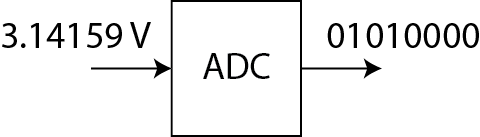
\includegraphics[width=\FigWidth\textwidth]{adc.png}
\caption{Analog-to-digital conversion: analog voltage input and binary number output.}
\label{f:adc}
\end{figure}
An important consideration of this ADC example is the resolution of the measurement, also known as the quantization error, which can be calculated using the same expression as before:
\begin{equation}
Q = \frac{FSR}{2^M} = \frac{\unit[10.0]{V}}{2^8} = \unit[39.1]{mV}.
\end{equation}
Because the ADC has 8-bits of resolution, it will report a binary number that is one of 256 possible levels.  Each level is separated by \unit[39.1]{mV} so that the total range is \unit[10.0]{V}.  If the actual input voltage is \unit[3.14159]{V} the ADC will report the closest binary level that correspond to this measurement which is $01010000$ (80 in decimal form).  So the ADC output, converted back to voltage, would be \unit[3.125]{V} $\pm$ \unit[0.0196]{V}, where \unit[0.0196]{V} is $Q/2$.  

Now if it wasn't bad enough that our 8-bit ADC has such coarse resolution, we also have to contend with the fact that the input voltage might be much smaller than the incoming range.  Consider what would happen if the actual input voltage only range between \unit[0--0.1]{V}, instead of the \unit[0--10.0]{V} range of the ADC.  In this case the ADC would only have four possible outputs corresponding to 0, 0.0391, 0.0782 and 0.1173 V.  So, in effect we would only be using 2-bits of our 8-bit ADC!

\begin{ex}
Consider an analog-to-digital converter with the following properties:
\begin{itemize}
\item FSR = $\pm$ \unit[1.0]{V}
\item 12-bit resolution
\end{itemize}
What is the resolution (in Volts) of the ADC?  
\end{ex}
\begin{ex}
Using the A/D converter described above, consider the case where the input to the ADC was exactly \unit[3.14]{V}. What binary number would be output by the ADC?
\end{ex}

\ifsolutions
\begin{soln}
\[ 
Q = \frac{2.0}{2^{12}} = \unit[0.0005]{V}
\]
The second part is a bit of a trick question.  Because the input is larger than the FSR, then the output would be the maximum value of the ADC - which is $2^{12}$ or 4,096.  
\end{soln}
\fi

\section{Summary}
The point of all this is the following:
\begin{itemize}
\item Digital representations of analog measurements have only finite resolution.
\item The input signal must be well matched to the ADC range to effectively use the full resolution of the ADC.  
\end{itemize}

So far we've just considered the simple idea of converting static analog measurement to a digital representation.  In the next chapter we'll consider what happens when we consider another dimension---time---in our understanding of measurement systems.  We'll also look at how to couple the ADC component with the rest of our system to make quality observations.

\section{Exercises}
\begin{ex}
Visit your favorite on-line vendor and search for a computer (PC or Mac) sound card.  Report the following specifications:
\begin{itemize}
\item Make and Model
\item Price
\item Audio input resolution (in bits)
\item Audio input range (in Volts)
\item Maximum sample rate (in Hz)
\end{itemize}
\end{ex}


